\documentclass[border=6pt]{standalone}
\usepackage{tikz}
\usepackage[edges]{forest}
\usetikzlibrary{arrows.meta,positioning,calc,decorations.pathreplacing,shapes.geometric}
\begin{document}
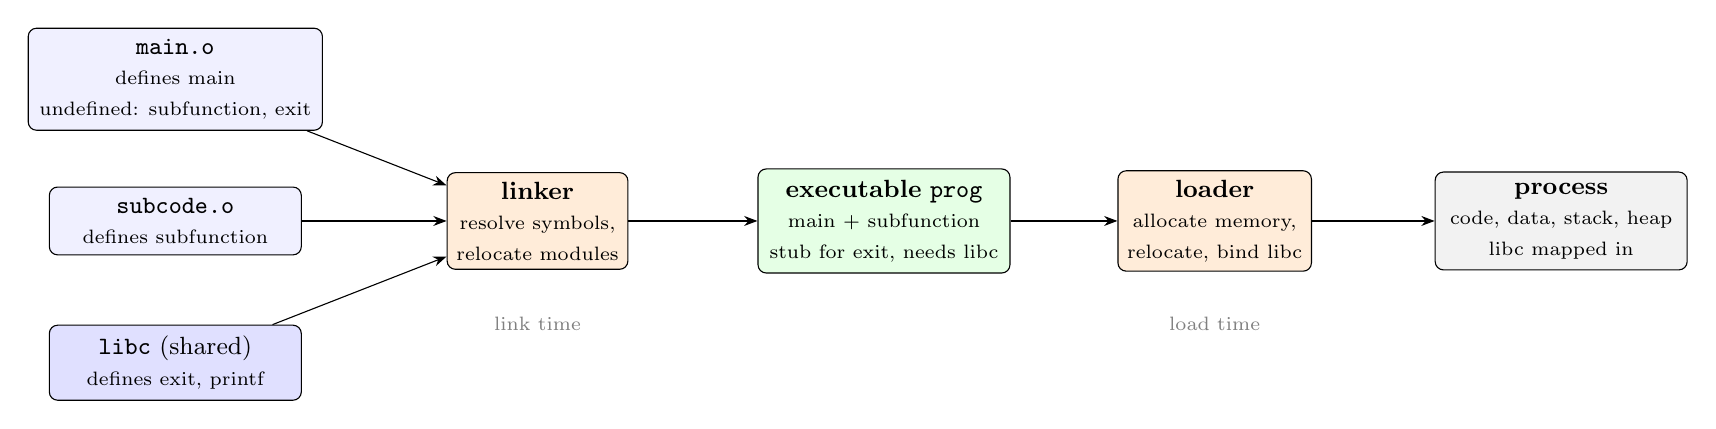
\begin{tikzpicture}[>=Stealth,font=\small,
 obj/.style={draw,rounded corners=3pt,fill=blue!6,align=center,minimum width=3.2cm,inner sep=4pt},
 pr/.style={draw,rounded corners=3pt,fill=orange!15,align=center,minimum width=2.2cm,minimum height=0.9cm}]
\node[obj] (m) at (0,1.8) {\texttt{main.o}\\{\scriptsize defines main}\\{\scriptsize undefined: subfunction, exit}};
\node[obj] (s) at (0,0) {\texttt{subcode.o}\\{\scriptsize defines subfunction}};
\node[obj,fill=blue!12] (l) at (0,-1.8) {\texttt{libc} (shared)\\{\scriptsize defines exit, printf}};
\node[pr] (ln) at (4.6,0) {\textbf{linker}\\{\scriptsize resolve symbols,}\\{\scriptsize relocate modules}};
\node[obj,fill=green!10] (ex) at (9.0,0) {\textbf{executable} \texttt{prog}\\{\scriptsize main + subfunction}\\{\scriptsize stub for exit, needs libc}};
\node[pr] (ld) at (13.2,0) {\textbf{loader}\\{\scriptsize allocate memory,}\\{\scriptsize relocate, bind libc}};
\node[obj,fill=gray!10] (pm) at (17.6,0) {\textbf{process}\\{\scriptsize code, data, stack, heap}\\{\scriptsize libc mapped in}};
\draw[->] (m)--(ln); \draw[->] (s)--(ln); \draw[->] (l)--(ln);
\draw[->] (ln)--(ex); \draw[->] (ex)--(ld); \draw[->] (ld)--(pm);
\node[font=\scriptsize,gray] at (4.6,-1.3) {link time}; \node[font=\scriptsize,gray] at (13.2,-1.3) {load time};
\end{tikzpicture}
\end{document}
